% !TEX program = xelatex
% 编译：在 slides/ 目录下运行 latexmk -xelatex slides.tex
% 图直接复用 ../figures/chN/*.pdf；内容与数字以 paper/ 为准，改正文后请同步核对。
\documentclass[aspectratio=169,11pt]{beamer}
\usepackage[UTF8,scheme=plain]{ctex}
\usetheme[progressbar=frametitle,numbering=none,sectionpage=progressbar,block=fill]{metropolis}

\usepackage{amsmath,amssymb,mathtools,bm}
\usepackage{booktabs,array,tabularx}
\usepackage[export]{adjustbox}
\usepackage[most]{tcolorbox}
\usepackage{pifont}
\usepackage{tikz}
\usetikzlibrary{arrows.meta,positioning,calc,shapes.symbols}
\graphicspath{{../figures/}}

% ---------------- 字体：有思源/Noto 黑体就用它（与图中字体一致），否则沿用 ctex 的默认（Windows 为微软雅黑） ----
% 西文：有 Inter 就用 Inter（引号、撇号是西文宽度），否则沿用默认无衬线字体
\IfFontExistsTF{Noto Sans CJK SC}{\setCJKsansfont{Noto Sans CJK SC}[BoldFont={* Bold}]}{%
  \IfFontExistsTF{Source Han Sans SC}{\setCJKsansfont{Source Han Sans SC}[BoldFont={* Bold}]}{}}
\IfFontExistsTF{Inter}{\setsansfont{Inter}}{}

% ---------------- 配色（与论文 preamble.tex、code/figstyle.py 一致）----------------
\definecolor{ink}{HTML}{0B0B0B}
\definecolor{inkMuted}{HTML}{52514E}
\definecolor{inkFaint}{HTML}{898781}
\definecolor{ruleGray}{HTML}{E1E0D9}
\definecolor{cBlue}{HTML}{2A78D6}
\definecolor{cOrange}{HTML}{EB6834}
\definecolor{cAqua}{HTML}{1BAF7A}
\definecolor{cYellow}{HTML}{EDA100}
\definecolor{cPink}{HTML}{E87BA4}
\definecolor{cViolet}{HTML}{6250D6}
\definecolor{cRed}{HTML}{E34948}
\definecolor{boxBack}{HTML}{F4F7FC}

\setbeamercolor{normal text}{fg=ink,bg=white}
\setbeamercolor{background canvas}{bg=white}
\setbeamercolor{alerted text}{fg=cOrange}
\setbeamercolor{example text}{fg=cAqua}
\setbeamercolor{frametitle}{fg=ink,bg=white}
\setbeamercolor{progress bar}{fg=cBlue,bg=ruleGray}
\setbeamercolor{title separator}{fg=cBlue}
\setbeamercolor{progress bar in section page}{fg=cBlue,bg=ruleGray}
\setbeamercolor{itemize item}{fg=cBlue}
\setbeamercolor{itemize subitem}{fg=inkFaint}
\setbeamercolor{enumerate item}{fg=cBlue}
\setbeamercolor{footline}{fg=inkFaint}
\setbeamercolor{subtitle}{fg=inkMuted}
\setbeamercolor{author}{fg=inkMuted}
\setbeamercolor{date}{fg=inkMuted}

\setbeamerfont{frametitle}{size=\large,series=\bfseries}
\setbeamerfont{title}{size=\LARGE,series=\bfseries}
\setbeamerfont{subtitle}{size=\large}
\setbeamerfont{section title}{size=\Large,series=\bfseries}
\setbeamerfont{footline}{size=\scriptsize}
\setbeamersize{text margin left=7mm,text margin right=7mm}
\setbeamertemplate{itemize item}[square]
\setbeamertemplate{itemize subitem}{\small\textendash}
\setbeamertemplate{enumerate item}{\insertenumlabel.}
\setlength{\leftmargini}{1.3em}
\AtBeginDocument{\setlength{\leftmargini}{1.3em}}
% 节标题页：比 metropolis 默认（22em）更宽，避免长标题折行
\makeatletter
\setbeamertemplate{section page}{%
  \centering
  \begin{minipage}{0.82\textwidth}
    \raggedright
    \usebeamercolor[fg]{section title}\usebeamerfont{section title}\insertsectionhead\\[-1ex]
    \usebeamertemplate*{progress bar in section page}
  \end{minipage}\par}
\makeatother

% 页脚：左侧当前部分名称，右侧页码
\newcommand{\footsec}{}
\newcommand{\setfootsec}[1]{\renewcommand{\footsec}{#1}}
\setbeamertemplate{footline}{%
  \begin{beamercolorbox}[wd=\paperwidth,ht=3.2ex,dp=1.6ex,leftskip=7mm,rightskip=7mm]{footline}%
    \usebeamerfont{footline}\footsec\hfill\insertframenumber\,/\,\inserttotalframenumber
  \end{beamercolorbox}}

% ---------------- 记号（与论文一致）----------------
\renewcommand{\emph}[1]{\textbf{#1}}
\newcommand{\Prob}{\mathbb{P}}
\newcommand{\E}{\mathbb{E}}
\newcommand{\Var}{\operatorname{Var}}
\newcommand{\Normal}{\mathcal{N}}
\newcommand{\dd}{\mathrm{d}}

% ---------------- 证据标签 ----------------
\newcommand{\evtag}[2]{\mbox{\textcolor{#1}{\scriptsize【#2】}}}
\newcommand{\tagLit}{\evtag{cBlue}{文献}}
\newcommand{\tagOff}{\evtag{cAqua}{官方}}
\newcommand{\tagPat}{\evtag{cViolet}{专利}}
\newcommand{\tagCom}{\evtag{cOrange}{社区}}
\newcommand{\tagOwn}{\evtag{cRed}{本项目}}

% ---------------- 版式小工具 ----------------
% 模拟参数、来源：小号墨灰色
\newcommand{\param}[1]{\par{\scriptsize\color{inkMuted}#1\par}}
\newcommand{\src}[1]{\par{\scriptsize\color{inkMuted}来源：#1\par}}
% 公式框
\newtcolorbox{eqbox}[1][]{enhanced,colback=boxBack,colframe=boxBack,boxrule=0pt,arc=2pt,
  left=5pt,right=5pt,top=2pt,bottom=2pt,before skip=2pt,after skip=4pt,before upper={\raggedright},#1}
% 要点框（左侧色条）
\newtcolorbox{notebox}[1][cBlue]{enhanced,colback=boxBack,colframe=boxBack,boxrule=0pt,arc=0pt,
  borderline west={2pt}{0pt}{#1},left=6pt,right=5pt,top=3pt,bottom=3pt,before skip=3pt,after skip=3pt}
% 数字卡片：\stat[颜色]{数字}{说明}
\newcommand{\stat}[3][cBlue]{%
  \begin{tcolorbox}[enhanced,colback=boxBack,colframe=boxBack,boxrule=0pt,arc=2pt,
    left=3pt,right=3pt,top=3pt,bottom=3pt,halign=center,valign=center,equal height group=stats,before skip=0pt,after skip=0pt]
    {\large\bfseries\color{#1}#2}\par\vspace{1pt}{\scriptsize\color{inkMuted}#3}
  \end{tcolorbox}}
% 截取多面板图的一部分：\crop{左 下 右 上（比例）}{尺寸选项}{文件}
\newcommand{\crop}[3]{\adjincludegraphics[trim={#1},clip,#2]{#3}}
% 列表间距
\newcommand{\tightlist}{\setlength{\itemsep}{2pt}\setlength{\parskip}{0pt}}
\newcommand{\looselist}{\setlength{\itemsep}{4pt}\setlength{\parskip}{0pt}}

\title{游戏中的 Elo 与匹配机制}
\subtitle{胜率能否计算、“Elo 感”从何而来、与模型训练的关系}
\author{DeepBattler 项目研究报告\texorpdfstring{\quad·\quad}{ · }论文配套幻灯片}
\date{2026 年 10 月}

\begin{document}

% =====================================================================
\setfootsec{}
{\vfuzz=20pt\maketitle}% metropolis 标题页的 \paperheight 小页总会报 overfull，这里只对标题页放宽

% =====================================================================
\setfootsec{问题与结论速览}
\begin{frame}{四个问题的答案：胜率能算，“Elo 感”无需操纵即可解释}
\footnotesize
\renewcommand{\arraystretch}{1.18}
\begin{tabularx}{\textwidth}{@{}>{\raggedright\arraybackslash}p{1.9cm}>{\raggedright\arraybackslash}p{3.6cm}>{\raggedright\arraybackslash}X@{}}
\toprule
& \textbf{提问者的问题} & \textbf{一句话回答} \\
\midrule
\textbf{\color{cBlue}研究一}\newline 文献与披露 & 通用和各游戏的 Elo、匹配有人研究吗？厂商披露过吗？有专利吗？ & \textbf{都有。}评分理论成熟；厂商普遍“隐藏分负责匹配、可见段位另算”，否认按连胜连败安排队友；EA 有以留存为目标的匹配专利与论文，但没有可复核的匹配日志。\\
\textbf{\color{cBlue}研究二}\newline 胜率能否计算 & 只有输赢、不干涉匹配，能算出胜率吗？和什么有关？ & \textbf{能算期望。}随机匹配下最强、最弱 10\% 约 83\% 与 17\%；按分匹配下恒等式把实力兑换成评分，长期胜率趋于 50\%；分辨 52\% 与 50\% 约需 4,900 局。\\
\textbf{\color{cBlue}研究三}\newline “Elo 感” & 诚实的系统会让人觉得被“控胜率”吗？ & \textbf{会，不需要操纵。}五成胜率打 100 局，81\% 会遇到 5 连败；诚实 Elo 的回归单局很小；真正放大连串的是连败触发的“上头”。\\
\textbf{\color{cBlue}研究四}\newline 训练视角 & target 是胜率还是实力？稳定后还有胜负数据吗？ & \textbf{标签是胜负，输出是胜率，潜参数是实力。}收敛后胜负像抛硬币，却是信息量最大的样本；检验要以冻结的收敛模型为零假设。\\
\bottomrule
\end{tabularx}
\end{frame}

% ---------------------------------------------------------------------
\begin{frame}{“每局五五开”是预测胜率五五开，不是实力五五开}
\begin{columns}[T,onlytextwidth]
\column{0.53\textwidth}
\small
“五五开”有三种读法，厂商的原话只支持第二种：
\begin{enumerate}\looselist
  \item[\textcolor{cRed}{\ding{55}}] \textbf{双方真实实力相等}\newline
    {\footnotesize\color{inkMuted}没有一家这样说：匹配器只看得到估计值 $R=s+e$}
  \item[\textcolor{cAqua}{\ding{51}}] \textbf{系统预测的单局胜率为 50\%}\newline
    {\footnotesize\color{inkMuted}Riot“50\%±1\%”、Dota 2“每队 50\% 的机会”、光环“50/50”}\tagOff
  \item[\textcolor{cRed}{\ding{55}}] \textbf{每个人的长期胜率为 50\%}\newline
    {\footnotesize\color{inkMuted}收敛的结果而非目标：光环称其为“副作用”，守望先锋称“不对任何人强制 50\% 胜率”}\tagOff
\end{enumerate}
\column{0.43\textwidth}
\begin{notebox}
\footnotesize
\textbf{预测 50\% 不等于真实 50\%}\par\smallskip
真实胜率 $p=F\big((R_A-R_B)-(e_A-e_B)\big)$ 围绕 50\% 分布：
\begin{itemize}\tightlist
  \item $K=16$：90\% 的“五五开”对局真实胜率在 \textbf{37.8\%–62.2\%}；$K=32$：33.2\%–66.8\% \tagOwn
  \item 5v5 两队评分和相等：随机对位的单挑 90\% 在 22\%–78\% \tagOwn
  \item 8 人局没有“五五开”：同分大厅前四率 50\%、第一 12.5\%、平均名次 4.5
\end{itemize}
\end{notebox}
\param{固定 $K$ 的 Elo 稳态，$\tau=200$；推导见论文研究二“每局五五开”一节。}
\end{columns}
\end{frame}

% =====================================================================
\setfootsec{研究一\quad 文献、厂商披露、专利与诉讼}
\section{研究一：文献、厂商披露、专利与诉讼}

\begin{frame}{评分与匹配是两层机制：“控胜率”若存在，只能在匹配层}
\begin{center}
\begin{tikzpicture}[
  box/.style={draw=none,fill=boxBack,rounded corners=2pt,align=center,text width=38mm,minimum height=15mm,inner sep=2.5pt,font=\footnotesize},
  arr/.style={-{Stealth[length=2.2mm]},thick,color=inkFaint}]
  \node[box] (r) {\textbf{\color{cBlue}评分模型}\\从胜负估计隐藏分 $R_i$\\{\scriptsize Elo、Glicko、TrueSkill}};
  \node[box,right=12mm of r] (m) {\textbf{\color{cOrange}匹配器}\\用 $R$、延迟、排队时间组局\\{\scriptsize 按分匹配、参与度匹配}};
  \node[box,right=12mm of m] (v) {\textbf{\color{cAqua}可见段位}\\段位、星数、外显分\\{\scriptsize 保底、进度分、追赶倍率}};
  \draw[arr] (r) -- node[above,font=\scriptsize,color=inkMuted]{$R$} (m);
  \draw[arr] (m.south) -- ++(0,-4mm) -| node[pos=0.25,below,font=\scriptsize,color=inkMuted]{对局结果 $y\in\{0,1\}$ 回到评分} (r.south);
  \draw[arr,dashed] (r.north) -- ++(0,3.5mm) -| node[pos=0.25,above,font=\scriptsize,color=inkMuted]{另算，不参与匹配} (v.north);
\end{tikzpicture}
\end{center}
\vspace{-1mm}
\begin{columns}[c,onlytextwidth]
\column{0.36\textwidth}
\begin{eqbox}
\small
$F(x)=\dfrac{1}{1+10^{-x/400}}$\\[2pt]
$E=F(R_i-R_j)$\\[2pt]
$R_i\leftarrow R_i+K\,(y-E)$\quad{\footnotesize\color{inkMuted}Elo 更新}
\end{eqbox}
\column{0.61\textwidth}
\footnotesize
\begin{itemize}\tightlist
  \item 评分是推断（估计实力 $s_i$），匹配是决策（选对手、分队）
  \item 分差 400 $\Rightarrow$ 期望得分 0.909；正态与逻辑斯蒂曲线相差不足 1.5 个百分点 \tagLit
  \item 玩家的指控常把三层混为一谈：可见段位的保底、加速被误认为匹配器在“安排”
\end{itemize}
\end{columns}
\end{frame}

% ---------------------------------------------------------------------
\begin{frame}{评分模型百年：逐条放松“两人、实力固定、一维”三个假设}
\begin{columns}[c,onlytextwidth]
\column{0.65\textwidth}
\centering
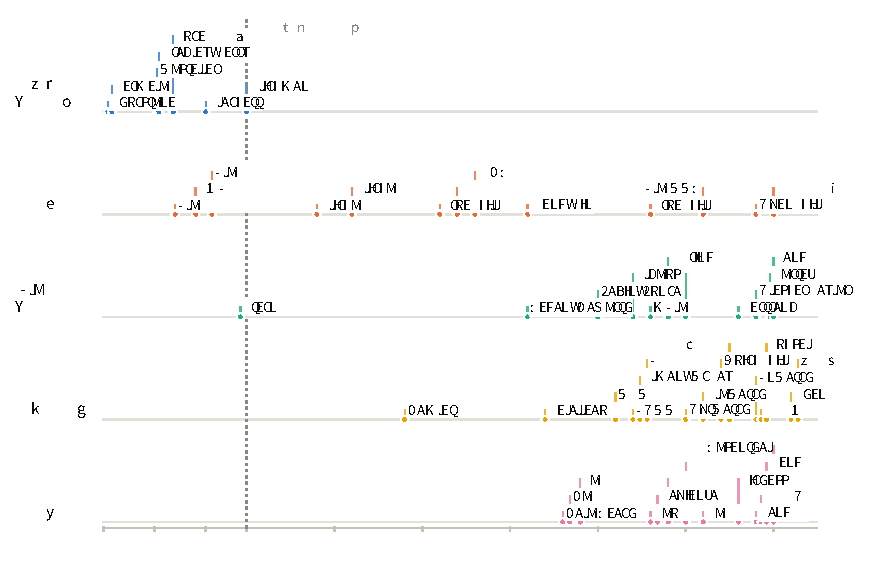
\includegraphics[height=69mm]{ch1/1a_timeline.pdf}
\column{0.33\textwidth}
\footnotesize
\begin{itemize}\looselist
  \item 成对比较 $\to$ Elo（USCF 1960、FIDE 1970）$\to$ Glicko 加误差棒 $\to$ TrueSkill 加团队与多人 $\to$ TTT/WHR 全历史平滑
  \item \textbf{修正错误假设收益最大}：TrueSkill 2 靠组排、经验、个人统计把《光环 5》准确率从 52\% 提到 68\% \tagLit
  \item \textbf{换公式收益很小}：KGS 围棋上 Elo 到 WHR 相差不到 0.7 个百分点 \tagLit
  \item 固定 $K$ 只能在“追得快”与“抖得小”间取舍；“约 30 场收敛”查无出处 \tagLit
\end{itemize}
\end{columns}
\end{frame}

% ---------------------------------------------------------------------
\begin{frame}{匹配研究的目标：公平即信息量最大，留存是另一回事}
\begin{columns}[T,onlytextwidth]
\column{0.40\textwidth}
\small
匹配研究里“最好”有四种含义：
\begin{enumerate}\looselist
  \item \textbf{公平}：结果最难预测，也对实力最有信息；TrueSkill 用“平局概率”定义匹配质量 \tagLit
  \item \textbf{等待}：总代价 $=$ 配对距离之和 $+$ 等待时间之和的在线匹配 \tagLit
  \item \textbf{分队}：均衡分队 NP 难；选位排队后在 3SUM 猜想下不可行 \tagLit
  \item \textbf{参与度}：EOMM 以预测流失为边权，求最小权完美匹配 \tagLit
\end{enumerate}
\column{0.57\textwidth}
\footnotesize
\textbf{以参与度为目标的研究：效应都不大}\par\smallskip
\renewcommand{\arraystretch}{1.25}
\begin{tabularx}{\linewidth}{@{}>{\raggedright\arraybackslash}p{2.2cm}>{\raggedright\arraybackslash}X@{}}
\toprule
研究 & 证据类型与结果 \\
\midrule
EOMM（EA） & 模拟：每轮留存 +0.3\%–1.1\%（均值 0.7\%）；常被引的“15\%”是 $1.007^{20}$ 的外推 \\
Chen 等 2026 & 模型反事实：参与度 +4\%–6\% \\
EnMatch（网易） & 两周 A/B：总对局数 +1.64\%、+7.19\% \\
CUPID（腾讯） & 30 天 A/B：5 分钟碾压率相对 −10.54\% \\
Yuksel 2024 & 合成数据：连胜 5 局后按“自己只有 1/12 $\approx$ 8\% 胜率”挑对手 \\
\bottomrule
\end{tabularx}
\par\smallskip
{\scriptsize\color{inkMuted}全部来自作者自有数据或自建模拟，本次检索没有找到独立复现。}
\end{columns}
\end{frame}

% ---------------------------------------------------------------------
\begin{frame}{厂商原话：被拉平的是预测胜率，长期 50\% 只是“副作用”}
\footnotesize
\renewcommand{\arraystretch}{1.1}
\begin{tabularx}{\textwidth}{@{}>{\raggedright\arraybackslash}p{2.3cm}>{\raggedright\arraybackslash}X>{\raggedright\arraybackslash}p{3.1cm}@{}}
\toprule
来源 & 原话（摘录，均出自官方开发者文章\tagOff） & 被拉平的量 \\
\midrule
Riot\newline 手游 2021 & ``MMR per team is balanced to give each team the same chance at winning the match (close to 50\%)'' & 两队 MMR，使预测胜率相等 \\
Riot\newline 英雄联盟 2025 & ``the team with more autofilled players will have slightly higher MMR players'' & 计入补位劣势后的预测胜率 \\
Valve\newline Dota 2 2017 & ``Simply having an even chance to win over the long run does not necessarily correlate to having competitive matches'' & 区分“长期均等”与“单局有悬念” \\
343\newline 光环 2022 & ``we expect to see an average 50\% win rate. Note that that's a side effect \ldots\ and not a goal'' & 单局预测胜率；长期 50\% 是副作用 \\
Blizzard\newline 酒馆战棋 2020 & ``we will try to select eight players with the closest internal rating'' & 8 人内部评分相近 \\
\bottomrule
\end{tabularx}
\par\smallskip
{\scriptsize\color{inkMuted}Riot 2018 年的“50\%±1\%”见前文；完整对照表见论文研究一“五五开”一节。\par}
\end{frame}

% ---------------------------------------------------------------------
\begin{frame}{专利：EA 的权利要求写明按“流失风险”组局，但专利不证明部署}
\footnotesize
\renewcommand{\arraystretch}{1.05}
\begin{tabularx}{\textwidth}{@{}>{\raggedright\arraybackslash}p{2.9cm}>{\raggedright\arraybackslash}p{1.6cm}>{\raggedright\arraybackslash}X>{\raggedright\arraybackslash}p{2.9cm}@{}}
\toprule
美国专利号 & 权利人 & 独立权利要求的通俗含义 & 部署证据 \\
\midrule
9,993,735 等 3 件 & EA & 匹配方案的“参与度分”（预测会继续玩的时长）低于阈值就换人 & 无 \\
10,286,327 等 3 件 & EA & 按两端玩家的流失风险给边加权、选边配对（EOMM 的骨架）& 无 \\
9,919,217 & EA & 预测流失率 $\to$ 调游戏“旋钮”（动态难度） & EA 称未用于 FIFA 等三款游戏 \\
9,789,406 & Activision & 按“对道具的兴趣 $+$ 对方持有该道具”匹配 & 公司称未实施 \\
7,050,868 等 & 微软 & TrueSkill 更新与配对；按实际与目标等待时间调阈值 & TrueSkill 公开部署 \\
\bottomrule
\end{tabularx}
\par\smallskip
\begin{notebox}[cViolet]
\footnotesize 读了 24 件美国授权专利的独立权利要求\tagPat：专利只说明“研究过并获得保护”，不说明已部署；中国专利全文未能检索。
\end{notebox}
\end{frame}

% ---------------------------------------------------------------------
\begin{frame}{两起诉讼都没有裁定“胜率是否被操纵”}
\begin{columns}[T,onlytextwidth]
\column{0.485\textwidth}
\begin{notebox}[cBlue]
\small\textbf{Zajonc 诉 EA（2020–2021）}\\[-1pt]
{\scriptsize\color{inkMuted}美国加州北区联邦地区法院，案号 3:20-cv-07871}
\end{notebox}
\footnotesize
\begin{itemize}\tightlist
  \item 原告指控 FIFA、Madden、NHL 的 Ultimate Team 未披露地使用动态难度调整（DDA）\tagCom
  \item 2021-02-11 原告自愿撤诉（不损害再诉权），EA 尚未答辩 \tagOff
  \item EA 声明：DDA 专利“从未用于 FIFA、Madden 或 NHL”，在线多人不用 DDA 给玩家优势或劣势 \tagOff
  \item 声明没有涉及 EA 的留存匹配专利家族
\end{itemize}
\column{0.485\textwidth}
\begin{notebox}[cOrange]
\small\textbf{孙千和诉腾讯（2024–2026）}\\[-1pt]
{\scriptsize\color{inkMuted}深圳市南山区人民法院，《王者荣耀》匹配机制}
\end{notebox}
\footnotesize
\begin{itemize}\tightlist
  \item 原告称连胜后会匹配到“很菜的队友和很强的对手”，直到胜率趋近 50\% \tagCom
  \item 请求公开匹配因素与权重；腾讯提交近 1000 页证据，主张技术秘密 \tagOff
  \item 腾讯展示的胜率：752 场 76.1\%、2398 场 71\%、472 场 81.6\%（样本由被告挑选）\tagOff
  \item 2026-04 公开的一审判决驳回全部请求：争点是“能否要求公开” \tagOff
\end{itemize}
\end{columns}
\medskip
\begin{notebox}[inkFaint]
\footnotesize 撤诉不是事实认定；判决既不能读作“证明了没有操纵”，也不能读作“默认了操纵”。
\end{notebox}
\end{frame}

% ---------------------------------------------------------------------
\begin{frame}{证据分三档：“研究过、申请过”已证实，“主流排位用没用”仍未知}
\footnotesize
\tcbset{evcol/.style={enhanced,colback=white,boxrule=0.6pt,arc=2pt,left=3pt,right=3pt,top=2pt,bottom=2pt,
  fonttitle=\small\bfseries,coltitle=white,equal height group=ev}}
\begin{columns}[T,onlytextwidth]
\column{0.32\textwidth}
\begin{tcolorbox}[evcol,colframe=cAqua,colbacktitle=cAqua,title={已证实}]
\begin{itemize}\tightlist
  \item EA 留存匹配专利；EOMM、EnMatch 论文
  \item EnMatch 部署于两款未具名游戏
  \item Activision 用 A/B 测试调技能约束、以留存评估
  \item 非实力规则：新手、回流、机器人、信誉、补位、组排
\end{itemize}
\end{tcolorbox}
\column{0.32\textwidth}
\begin{tcolorbox}[evcol,colframe=cOrange,colbacktitle=cOrange,title={被否认（公司自述）}]
\begin{itemize}\tightlist
  \item 读取连胜连败安排队友、输家队列
  \item 强制 50\% 胜率
  \item 按消费匹配
  \item EA 在线多人用 DDA（唯一经诉讼间接检验）
  \item 《漫威争锋》使用 EOMM
\end{itemize}
\end{tcolorbox}
\column{0.32\textwidth}
\begin{tcolorbox}[evcol,colframe=inkMuted,colbacktitle=inkMuted,title={仍然未知}]
\begin{itemize}\tightlist
  \item 主流排位是否逐局使用流失预测
  \item 未公开 A/B 测试的时段与配置
  \item 《王者荣耀》等的评分模型与“表现分”权重
  \item \textbf{没有任何厂商公开可复核的匹配日志}
\end{itemize}
\end{tcolorbox}
\end{columns}
\smallskip
\begin{notebox}
\footnotesize 能定论的是数据：逐局隐藏分与系统预测——控制自身评分后，近期连胜连败还能否预测对手和队友的评分。
\end{notebox}
\end{frame}

% =====================================================================
\setfootsec{研究二\quad 不干涉匹配时，胜率能否计算}
\section{研究二：不干涉匹配时，胜率能否计算}

\begin{frame}{实力、评分、胜率是三个量：同一实力换个对手池，胜率就变}
\begin{columns}[c,onlytextwidth]
\column{0.55\textwidth}
\centering
\crop{0 0 {.392\width} 0}{height=62mm}{ch2/three_quantities.pdf}
\column{0.43\textwidth}
\begin{eqbox}\small
$W(s;\mathcal G)=\displaystyle\int F(s-t)\,\dd\mathcal G(t)$\\[1pt]
{\footnotesize\color{inkMuted}胜率 $=$ 实力对\emph{实际}对手分布的平均}
\end{eqbox}
\footnotesize
\begin{itemize}\looselist
  \item 同一实力 $s=1756$（第 90 百分位）：随机匹配下 80.0\%（$\tau=100$）$\to$ 73.2\%（$\tau=300$）；按分匹配下 64.5\% $\to$ 50.9\%（窗口收窄）
  \item 评分是带噪声、滞后、刻度的估计：按分匹配稳态下与实力相关 0.986，但斜率 $\lambda=1.19$、残差 41 分
  \item 可操作的定义：实力 $=$ 对固定参照池的胜率
\end{itemize}
\end{columns}
\param{10,000 人，$s\sim\Normal(1500,\tau^2)$，$K=16$，3000 轮，统计第 1001–3000 局；$s=1756$ 为 $\tau=200$ 群体的第 90 百分位。\tagOwn}
\end{frame}

% ---------------------------------------------------------------------
\begin{frame}{“五五开”的一局，真实胜率在 38\%–62\% 之间（$K=16$）}
\begin{columns}[c,onlytextwidth]
\column{0.62\textwidth}
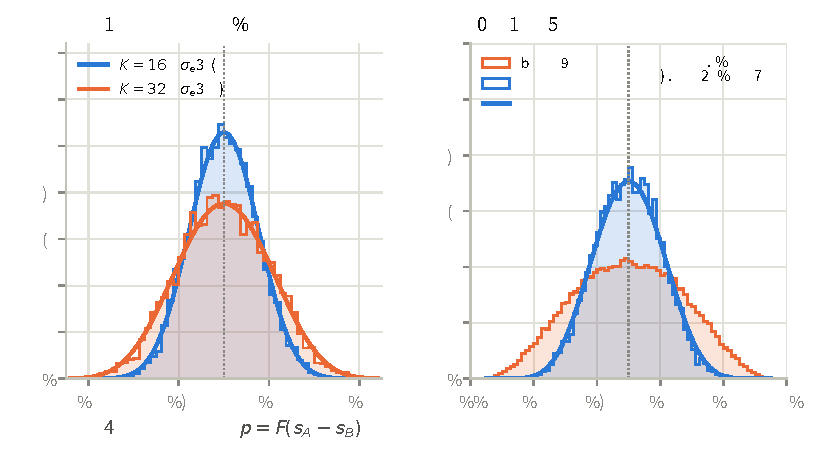
\includegraphics[width=\linewidth]{ch2/fair_game.pdf}
\column{0.36\textwidth}
\begin{eqbox}\footnotesize
$(s_A-s_B)\mid R_A{=}R_B\sim\Normal(0,\sigma_\Delta^2)$\\[2pt]
$\sigma_\Delta^2=\dfrac{2\tau^2\sigma_e^2}{\tau^2+\sigma_e^2}$，\ $p=F(s_A-s_B)$
\end{eqbox}
\footnotesize
\begin{itemize}\tightlist
  \item $K=16$：$\sigma_e=37.7$，$\sigma_\Delta=52.4$；90\% 落在 37.8\%–62.2\%，平均偏离 5.9 个百分点
  \item $K=32$：33.2\%–66.8\%
  \item 5v5 团队 32\%–68\%；随机对位的单挑 22\%–78\%，约 26\% 偏离 50\% 超过 20 个百分点
\end{itemize}
\end{columns}
\param{评分表取自随机匹配模拟第 3000 轮（10,000 人，$\tau=200$）；(b) 加和模型、$K=16$，按 $R+\Normal(0,100^2)$ 每 10 人一局，在 126 种分队中取评分和最接近者。\tagOwn}
\end{frame}

% ---------------------------------------------------------------------
\begin{frame}{随机匹配：胜率只由实力百分位和运气比例决定}
\begin{columns}[c,onlytextwidth]
\column{0.45\textwidth}
\centering
\crop{0 0 {.464\width} 0}{height=61mm}{ch2/random_1v1.pdf}
\column{0.53\textwidth}
\begin{eqbox}\footnotesize
$W(s)=\Phi\Big(\dfrac{s-\mu}{\sqrt{\sigma_d^2+\tau^2}}\Big)=\Phi(r\,z_q),\quad r=\dfrac{\tau}{\sqrt{\tau^2+\sigma_d^2}}$\\[1pt]
{\color{inkMuted}$z_q$：实力百分位的正态分位数；$\sigma_d\approx295.7$ 使 $F(d)\approx\Phi(d/\sigma_d)$}
\end{eqbox}
\footnotesize
\begin{itemize}\looselist
  \item $\tau=200$：十分位胜率 17.0\% $\to$ 82.9\%；前 1\% 为 92.7\%（公式 92.5\%）
  \item 群体越分散越极端：前 10\% 由 71.7\%（$\tau=100$）到 88.2\%（$\tau=300$）
  \item 单局越随机越接近 50\%：单局噪声 $\sigma_x=150$ 时最强 10\% 从 82.9\% 降到 79.4\%；$K$ 不影响随机匹配的胜率
\end{itemize}
\end{columns}
\param{点为模拟（10,000 人，$K=16$，随机配对，3000 轮，统计第 1001–3000 局），曲线为公式。\tagOwn}
\end{frame}

% ---------------------------------------------------------------------
\begin{frame}{按分匹配把实力兑换成评分，长期胜率被压向 50\%}
\begin{columns}[c,onlytextwidth]
\column{0.45\textwidth}
\centering
\crop{0 0 {.508\width} 0}{height=61mm}{ch2/sbmm_deciles.pdf}
\column{0.53\textwidth}
\begin{eqbox}\small
$W_T\equiv\dfrac1T\displaystyle\sum_{t=1}^T y_t=\bar E_T+\dfrac{R_T-R_0}{K\,T}$\\[1pt]
{\footnotesize\color{inkMuted}固定 $K$ 的 Elo 的代数恒等式，对任何匹配方式都精确成立}
\end{eqbox}
\footnotesize
\begin{itemize}\looselist
  \item 偏离 50\% 只有两个来源：对手系统性更弱或更强（$\bar E\ne\tfrac12$）；评分仍在单向移动（新号、进步）
  \item 十分位胜率：随机 17.0\%–82.9\%；$\sigma_q=200$ 时 30.9\%–69.1\%；$\sigma_q=100$ 时 42.1\%–58.0\%；$\sigma_q=20$ 时 48.8\%–51.2\%
  \item 天梯两端人少、窗口对称而人口不对称，所以仍偏离 50\%——不是操纵
\end{itemize}
\end{columns}
\param{10,000 人，$\tau=200$，$K=16$，按 $R+\Normal(0,\sigma_q^2)$ 排序相邻配对，3000 轮，统计第 1001–3000 局。\tagOwn}
\end{frame}

% ---------------------------------------------------------------------
\begin{frame}{段位与分数只通过对手起作用：重置到 1500 的高手前 50 局胜率 77.5\%}
\begin{columns}[c,onlytextwidth]
\column{0.45\textwidth}
\centering
\crop{{.50\width} 0 0 0}{height=61mm}{ch2/reset.pdf}
\column{0.53\textwidth}
\footnotesize
\begin{itemize}\looselist
  \item 评分落后实力约 350 分：按分匹配追回一半要 47 局（$K=16$）/ 30 局（$K=32$），追回 90\% 要 150 / 96 局
  \item 前 50 局胜率 77.5\% / 73.6\%，第 301–400 局回落到 58.9\% / 57.1\%，即前 10\% 玩家在该窗口下的平稳胜率
  \item 随机匹配下胜率与评分无关，始终约 83\%
  \item 可见段位叠加保底与加分，不满足 $K(y-E)$，不宜直接用来估计实力；守望先锋 2、酒馆战棋都只用隐藏分匹配 \tagOff
\end{itemize}
\end{columns}
\param{系统运行 1000 轮后，从实力前 10\% 中随机抽 500 人把评分重置为 1500；10,000 人，$\tau=200$，按分匹配 $\sigma_q=100$ 或随机匹配；10 局滑动平均。\tagOwn}
\end{frame}

% ---------------------------------------------------------------------
\begin{frame}{团队稀释个人优势：约按 $1/\sqrt n$（加和模型）到 $1/n$（均值模型）}
\begin{columns}[c,onlytextwidth]
\column{0.45\textwidth}
\centering
\crop{0 0 {.462\width} 0}{height=61mm}{ch2/team.pdf}
\column{0.53\textwidth}
\begin{eqbox}\footnotesize
$W_{\text{加和}}\approx\Phi\Bigg(\dfrac{d/\sqrt n}{\sqrt{\sigma_d^2+(2n-1)\tau^2/n}}\Bigg)$\\[2pt]
$W_{\text{均值}}\approx\Phi\Bigg(\dfrac{d/n}{\sqrt{\sigma_d^2+(2n-1)\tau^2/n^2}}\Bigg)$
\end{eqbox}
\footnotesize
\begin{itemize}\looselist
  \item 两层稀释：个人优势只占团队差的 $1/\sqrt n$ 或 $1/n$；队友和对手的离散 $(2n-1)\tau^2$ 又加一层噪声
  \item $n=5$：斜率为 1v1 的 0.40（加和）或 0.23（均值）
  \item 最强 10\%：1v1 83.1\%，5v5 65.2\%（加和）/ 59.0\%（均值）
  \item 随机分队的 5v5，个人长期胜率的标准差 8.8 个百分点（1v1 为 19.6）
\end{itemize}
\end{columns}
\param{图为加和模型：焦点玩家比群体平均高 $d$ 分，队友和对手随机；曲线为精确数值积分，点为模拟（$\tau=200$，10,000 人，$K=16$）。\tagOwn}
\end{frame}

% ---------------------------------------------------------------------
\begin{frame}{8 人局的基准取决于“胜”的定义：第一名 12.5\%，前四 50\%}
\begin{columns}[c,onlytextwidth]
\column{0.45\textwidth}
\centering
\crop{0 0 {.487\width} 0}{height=61mm}{ch2/ffa.pdf}
\column{0.53\textwidth}
\begin{eqbox}\footnotesize
Plackett–Luce，$w=10^{d/400}$，$N=8$：\\[2pt]
$\Prob(\text{第 1})=\dfrac{w}{w+N-1}$\\[2pt]
$\Prob(\text{前 }k)=1-\displaystyle\prod_{j=0}^{k-1}\frac{N-1-j}{w+N-1-j}$
\end{eqbox}
\footnotesize
\begin{itemize}\looselist
  \item 比其余 7 人强 100 分：第一 20.3\%、前四 68.6\%、平均名次 3.52；强 200 分：31.1\%、84.6\%、2.68
  \item 按分匹配（$\sigma_q=100$）下最强 10\%：第一 17.0\%、前四 61.3\%、平均名次 3.90
  \item 一局给出 7 组比较，评分误差更小：$K=16$ 时 24.7 分（1v1 为 37.8）
\end{itemize}
\end{columns}
\param{表现 $=$ 实力 $+$ Gumbel 噪声；点为蒙特卡洛（每点 20 万局）；人群模拟 10,000 人，两两 Elo 更新每对步长 $K/7$。\tagOwn}
\end{frame}

% ---------------------------------------------------------------------
\begin{frame}{实力有波动时期望仍可算，但窗口胜率比二项分布更分散}
\begin{columns}[c,onlytextwidth]
\column{0.45\textwidth}
\centering
\crop{{.527\width} 0 0 0}{height=61mm}{ch2/ar1.pdf}
\column{0.53\textwidth}
\begin{eqbox}\footnotesize
评分吸收的状态份额 $a=\dfrac{b\rho}{1-(1-b)\rho}$；期望胜率\\[2pt]
$W(t)\approx\bar E(t)+\dfrac{\lambda v(t)}{K}+\dfrac c4(1-a)\,u_t$
\end{eqbox}
\footnotesize
\begin{itemize}\looselist
  \item AR(1) 状态：评分吸收约 63\%（$K=16$）；没吸收的部分照样进入胜率，手热时 58.9\%、手冷时 41.1\%
  \item 百局胜率方差 $/$ 二项方差：随机 $+$ 状态 3.60，按分 $+$ 状态 1.61，按分且实力固定 0.56
  \item 持续进步 0.5 分/局：胜率高出期望 3.54 个百分点（$\approx\lambda v/K$）
\end{itemize}
\end{columns}
\param{AR(1) 状态 $\sigma_u=100$，$\rho=0.99$；按分匹配 $\sigma_q=100$，$K=16$；10,000 人，$\tau=200$，3000 轮；点为模拟，曲线为公式。\tagOwn}
\end{frame}

% ---------------------------------------------------------------------
\begin{frame}{区分 52\% 与 50\% 约需 4,900 局；8 人局用完整名次更省样本}
\begin{columns}[c,onlytextwidth]
\column{0.45\textwidth}
\centering
\crop{{.49\width} 0 0 0}{height=61mm}{ch2/ci.pdf}
\column{0.53\textwidth}
\begin{eqbox}\footnotesize
\centering $n=\Bigg(\dfrac{z_{1-\alpha/2}\sqrt{p_0(1-p_0)}+z_{1-\beta}\sqrt{p_1(1-p_1)}}{p_1-p_0}\Bigg)^{2}$
\end{eqbox}
\footnotesize
\begin{itemize}\looselist
  \item 52\% 对 50\%：4,903 局（双侧 5\%，检验力 80\%）
  \item 100 局的标准误 $\pm5.00$ 个百分点；真实 50\% 时 100 局胜率 $\ge60\%$ 的概率 2.84\%——玩家一多，总有人凭运气打出漂亮战绩
  \item 8 人局同等优势：第一名率约 17,700 局，平均名次约 3,400 局；估计实力应优先用完整名次
\end{itemize}
\end{columns}
\param{各局独立的正态近似；8 人局按 Plackett–Luce 换算到相同的实力优势（前四率 52\% 对应 $d\approx11$ 分）。\tagOwn}
\end{frame}

% =====================================================================
\setfootsec{研究三\quad 诚实系统会不会制造“Elo 感”}
\section{研究三：诚实系统会不会制造“Elo 感”}

\begin{frame}{纯随机已足以制造长连败：五成胜率打 100 局，81\% 会遇到 5 连败}
\begin{columns}[c,onlytextwidth]
\column{0.47\textwidth}
\centering
\crop{0 {.17\height} {.463\width} 0}{width=\linewidth}{ch3/longest_run.pdf}
\column{0.51\textwidth}
\begin{eqbox}\small
最长连败的 Gumbel 近似 \tagLit：\\[2pt]
$\E L_n\approx\log_{1/q}(np)+\dfrac{\gamma}{\ln(1/q)}-\dfrac12$
\end{eqbox}
\footnotesize
\begin{itemize}\looselist
  \item 100 局：最长连败期望 5.99 局；1000 局内出现 10 连败的概率 39\%（胜率 45\% 时 68\%）
  \item 1000 万名五成玩家各打 500 局：约 21\%（两百多万人）会遇到 $\ge10$ 连败
  \item 一晚打 20 局，出现 $\ge4$ 连败的概率 48\%
\end{itemize}
\end{columns}
\param{各局独立，单局胜率 50\%；实线为马尔可夫链精确值，虚线为泊松近似。\tagOwn}
\end{frame}

% ---------------------------------------------------------------------
\begin{frame}{“连胜紧接连败”和低谷窗口同样常见，不需要任何安排}
\begin{columns}[c,onlytextwidth]
\column{0.47\textwidth}
\centering
\crop{0 0 {.467\width} 0}{width=\linewidth}{ch3/pattern_window.pdf}
\column{0.51\textwidth}
\begin{eqbox}\small
“$\ge k$ 连胜紧接 $\ge k$ 连败”的期望次数（精确）：\\[2pt]
$\E N_{k}=(n-2k+1)\,(pq)^k$
\end{eqbox}
\footnotesize
\begin{itemize}\looselist
  \item “4 连胜紧接 4 连败”：100 局内 31\%，1000 局内 98\%
  \item “5 接 5”：100 局内 8.6\%，1000 局内 62\%
  \item 不必连续：100 局里 78\% 会出现某 10 局只赢 $\le2$ 局，56\% 会出现某 20 局只赢 $\le6$ 局
  \item 主观的“连胜后连败”往往不要求两段紧挨着，体感频率更高
\end{itemize}
\end{columns}
\param{单局胜率 50\%，各局独立；“至少出现一次”用 KMP 自动机动态规划精确计算。\tagOwn}
\end{frame}

% ---------------------------------------------------------------------
\begin{frame}{自查战绩的陷阱：独立序列里“3 连胜后胜率”的期望只有 46.0\%}
\begin{columns}[c,onlytextwidth]
\column{0.47\textwidth}
\centering
\crop{0 0 {.504\width} 0}{height=60mm}{ch3/ms_bias.pdf}
\column{0.51\textwidth}
\footnotesize
\textbf{Miller–Sanjurjo 偏差} \tagLit
\begin{eqbox}\footnotesize
$\E\big[\hat P_1\mid N_1=n_1\big]=\dfrac{n_1-1}{n-1}<\dfrac{n_1}{n}$
\end{eqbox}
自查最近 100 局：3 连胜后 46.0\%、4 连胜后 41.3\%、5 连胜后 36.5\%——恰好像“系统在惩罚连胜” \tagOwn
\par\medskip
\textbf{全服合并的构成效应}
\begin{eqbox}\footnotesize
$\Prob(\text{胜}\mid\text{最近 }k\text{ 局全胜})=\dfrac{\E[p^{k+1}]}{\E[p^k]}\ge\E[p]$
\end{eqbox}
随机匹配下“5 连胜后”73.7\%、“5 连败后”26.3\%，而同一玩家内部毫无变化 \tagOwn
\end{columns}
\param{单局胜率 50\%，精确动态规划；构成效应取实力 $\Normal(0,200^2)$。检验应合并计数、做玩家内置换，或扣除算出的偏差。}
\end{frame}

% ---------------------------------------------------------------------
\begin{frame}{诚实 Elo 自带均值回归：5 连胜后下一局约低 3 个百分点（1v1，$K=32$）}
\begin{columns}[c,onlytextwidth]
\column{0.47\textwidth}
\centering
\crop{0 0 {.928\width} 0}{height=50mm}{ch3/elo_reversion.pdf}%
\crop{{.535\width} 0 0 0}{height=50mm}{ch3/elo_reversion.pdf}
\column{0.51\textwidth}
\begin{eqbox}\footnotesize
评分过冲约 $kK/4$，下一局胜率超额：\\[2pt]
$\Delta_k\approx-\dfrac{\kappa\,c\,K\,k}{16\,n}$\quad{\footnotesize\color{inkMuted}（$n$ 为每队人数）}
\end{eqbox}
\footnotesize
\begin{itemize}\looselist
  \item 5 连胜后：1v1 $K=10$ 为 $-1.2$、$K=32$ 为 $-3.0$；5v5 为 $-0.5$（均值模型）/ $-0.9$（加和模型）个百分点
  \item 按近期战绩更明显：前 20 局 14 胜 6 负后约 $-4.3$ 个百分点
  \item 连败使对手变弱，长连败反而更少：千局 $\ge10$ 连败 40.5\% $\to$ 29.3\%（这是诚实系统的预测，不是操纵）
\end{itemize}
\end{columns}
\param{闭合人群 10,000 人，实力 $\Normal(0,200^2)$，预热 1500 轮后记录 2000 局；1v1 $\sigma_q=100$；5v5 随机分队、$\sigma_q=250$；$\kappa$ 取实力对评分的回归斜率。点为模拟，线为线性高斯近似。\tagOwn}
\end{frame}

% ---------------------------------------------------------------------
\begin{frame}{把“状态”写成 $s_t=s+u_t$：五种实力波动模型，区别在时间尺度}
\footnotesize
\begin{columns}[T,onlytextwidth]
\column{0.49\textwidth}
\begin{itemize}\tightlist
  \item[(a)] 逐局独立噪声：$u_t\sim\Normal(0,\sigma_u^2)$，$\sigma_u=100$
  \item[(b)] AR(1) 状态：$u_t=\rho u_{t-1}+\varepsilon_t$，$\rho=0.9$，$\sigma_u=60$
  \item[(c)] 两状态：状态差时 $u=-120$，平均持续 10 局
\end{itemize}
\column{0.49\textwidth}
\begin{itemize}\tightlist
  \item[\textbf{(d)}] \textbf{上头}：$u_t=-\theta\min(L_{t-1},m)$，$\theta=30$，$m=3$；$L$ 为当前连败，赢一局或休息后归零
  \item[(e)] 疲劳：$u_t=-\psi\,(j_t-1)$，$\psi=6$；$j_t$ 为本次游玩第几局
\end{itemize}
\end{columns}
\par\smallskip
\centering
\crop{0 {.783\height} 0 {.013\height}}{width=0.74\textwidth}{ch3/models_traj.pdf}\\[-1pt]
\crop{0 {.365\height} 0 {.434\height}}{width=0.74\textwidth}{ch3/models_traj.pdf}\\
{\scriptsize\color{inkMuted}\textcolor{cBlue}{\rule[0.5ex]{4mm}{1pt}} 有效实力偏离 $u_t$\quad \textcolor{cOrange}{\rule[0.5ex]{4mm}{1pt}} 评分 $R_t$（相对平均实力）\quad 顶部短线：每局胜（上）/ 负（下）；单人、校准对手池、Elo $K=20$\par}
\end{frame}

% ---------------------------------------------------------------------
\begin{frame}{上头：连败触发的自激，把一次普通的失败放大成一串}
\begin{columns}[c,onlytextwidth]
\column{0.47\textwidth}
\centering
\crop{0 0 {.493\width} 0}{height=57mm}{ch3/tilt_chain.pdf}
\column{0.51\textwidth}
\begin{eqbox}\small
$u_t=-\theta\,\min(L_{t-1},m)$\qquad{\footnotesize\color{inkMuted}$\theta=30$，$m=3$}\\[1pt]
{\footnotesize\color{inkMuted}继续输的概率：50\% $\to$ 54\% $\to$ 58\% $\to$ 62\%}
\end{eqbox}
\begin{columns}[T,onlytextwidth]
\column{0.485\linewidth}
\stat[cYellow]{+86\%–97\%}{“5 连胜紧接 5 连败”}\par\smallskip
\stat[cYellow]{6.3\% $\to$ 12.3\%}{一段连败 $\ge5$ 局}
\column{0.485\linewidth}
\stat[cYellow]{39\% $\to$ 64\%}{千局内 $\ge10$ 连败（Elo）}\par\smallskip
\stat[cAqua]{+70\%}{有休息时的“5 接 5”（无休息 +86\%）}
\end{columns}
\end{columns}
\param{单人对校准对手池（$\sigma_q=50$），评分不动（图，精确马尔可夫链）或 Elo $K=20$（模拟，$2\times10^4$ 人 $\times$ 1000 局）；“5 接 5”相对玩家内打乱基线。\tagOwn}
\end{frame}

% ---------------------------------------------------------------------
\begin{frame}{评分吸收慢状态，只有上头显著放大长连败和“连胜后连败”}
\begin{columns}[T,onlytextwidth]
\column{0.55\textwidth}
\footnotesize
\textbf{评分按 Elo 更新（$K=20$）时的统计痕迹}\par\smallskip
\renewcommand{\arraystretch}{1.2}
\begin{tabular}{@{}lccc@{}}
\toprule
模型 & 千局 $\ge10$ 连败 & 4 接 4 & 5 接 5 \\
     & {\scriptsize 实际 / 打乱} & & \\
\midrule
无波动 & 0.256 / 0.380 & +4\% & +6\% \\
(b) AR(1) & 0.413 / 0.380 & +4\% & +10\% \\
(c) 两状态 & 0.366 / 0.382 & +4\% & +7\% \\
\textbf{(d) 上头} & \textbf{0.644 / 0.391} & \textbf{+55\%} & \textbf{+97\%} \\
(d$'$) 上头 $+$ 休息 & 0.554 / 0.375 & +45\% & +73\% \\
(e) 疲劳 & 0.361 / 0.377 & +4\% & +6\% \\
\bottomrule
\end{tabular}
\column{0.42\textwidth}
\begin{eqbox}\footnotesize
胜率中残留的状态方差比例：\\[2pt]
$\dfrac{\Var D_t}{\sigma_u^2}\approx\dfrac{1-\rho}{(1-\rho)+b}$
\end{eqbox}
\footnotesize
\begin{itemize}\looselist
  \item 状态记忆约 $1/(1-\rho)$ 局，评分记忆约 $1/b\approx35$ 局：$\rho=0.9$ 保留 81\%，0.98 保留 42\%，0.99 保留 26\%
  \item 上头发生在评分来不及反应的几局之内，几乎不被吸收
  \item 慢状态与诚实回归方向相反、可以抵消：“连胜后约五成”不能说明“没有状态”
\end{itemize}
\end{columns}
\param{单人校准对手池，$\sigma_q=50$，$2\times10^4$ 名玩家 $\times$ 1000 局；“4 接 4”“5 接 5”为“$\ge k$ 连胜紧接 $\ge k$ 连败”的次数相对玩家内打乱基线的变化；$b=cK/4\approx0.029$。\tagOwn}
\end{frame}

% ---------------------------------------------------------------------
\begin{frame}{操纵若存在，指纹在匹配输入里：连胜后对手评分高出 71–79 分}
\begin{columns}[c,onlytextwidth]
\column{0.47\textwidth}
\centering
\crop{{.50\width} {.205\height} 0 0}{height=50mm}{ch3/manip.pdf}\\[1pt]
{\scriptsize\color{inkMuted}\textcolor{cBlue}{\rule[0.5ex]{4mm}{1pt}} 诚实 Elo（与上头几乎重合）\quad
\textcolor{cAqua}{\rule[0.5ex]{4mm}{1pt}} 对称操纵：连胜 $\ge3$ 配 $+100$、连败 $\ge3$ 配 $-100$\quad
\textcolor{cYellow}{\rule[0.5ex]{4mm}{1pt}} 只对连胜 $\ge3$ 配 $+100$\par}
\column{0.51\textwidth}
\footnotesize
\begin{itemize}\looselist
  \item \textbf{对手评分差}（5 连胜后）：对称控五成 +78.5、只惩罚连胜 +70.9；诚实 Elo −3.7（对手\emph{真实}实力 +22.8：是你的评分虚高）
  \item \textbf{阈值处的断崖}：诚实回归随连胜长度平滑；操纵在触发长度处跳变
  \item \textbf{长连败方向}：控五成反而减少长连败（千局 $\ge10$ 连败 12\% 对 41\%）；“输家队列”只有叠加上头才放大连串
\end{itemize}
\begin{notebox}[cOrange]
\footnotesize\textbf{推荐检验}：对手评分 $-$ 我方评分 $\sim$ 近期连胜、连败指示变量 $+$ 自身评分、排队时间、时段、组队人数 $+$ 玩家固定效应。只看胜负，最多能说“没有发现强操纵”。
\end{notebox}
\end{columns}
\param{人群模拟：1v1，$K=32$，$\sigma_q=100$，10,000 人，记录 2000 局/人；图为对手评分减我方评分的玩家内部超额，虚线为触发阈值 $\pm3$。\tagOwn}
\end{frame}

% ---------------------------------------------------------------------
\begin{frame}{酒馆战棋：夺冠率 1/8 时，100 局里 60\% 的人会遇到 $\ge20$ 局无冠}
\begin{columns}[c,onlytextwidth]
\column{0.58\textwidth}
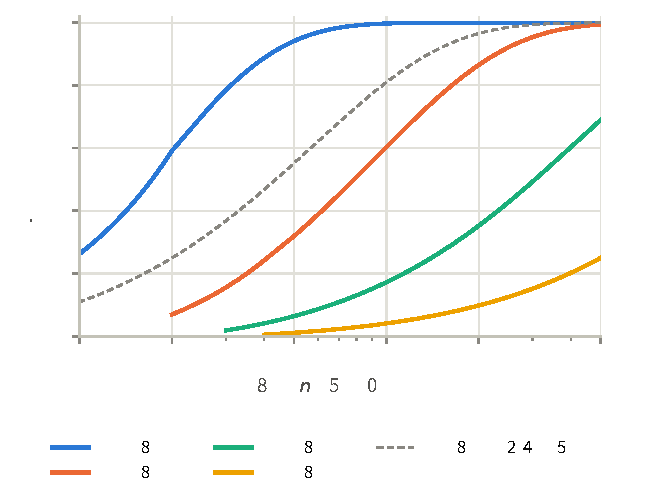
\includegraphics[width=\linewidth]{ch3/bg_drought.pdf}
\column{0.40\textwidth}
\small
\begin{itemize}\looselist
  \item 前四是一枚公平硬币：100 局里 81\% 的人会遇到 $\ge5$ 局连续后四
  \item 100 局：$\ge10$ 局无冠 99.8\%，$\ge20$ 局 60.3\%，$\ge30$ 局 17.2\%；最长无冠段期望 22.8 局
  \item 500 局：$\ge30$ 局无冠的概率 69\%
  \item 诚实回归与上头同样存在；外显分的地板和追赶倍率只影响显示，不影响匹配 \tagOff
\end{itemize}
\end{columns}
\param{同分大厅、夺冠率 1/8、各局独立，精确计算。判断版本好坏要看足够多局的名次分布，而不是最近一段的体感。\tagOwn}
\end{frame}

% =====================================================================
\setfootsec{研究四\quad 训练视角：目标是胜率还是实力}
\section{研究四：训练视角——目标是胜率还是实力}

\begin{frame}{标签是胜负，输出是胜率，被学到的是实力}
\begin{columns}[c,onlytextwidth]
\column{0.60\textwidth}
\footnotesize
\renewcommand{\arraystretch}{1.3}
\begin{tabularx}{\linewidth}{@{}>{\raggedright\arraybackslash}p{1.9cm}>{\raggedright\arraybackslash}p{1.75cm}>{\raggedright\arraybackslash}p{1.85cm}>{\raggedright\arraybackslash}X@{}}
\toprule
场景 & 训练标签 & 模型输出 & 被学到的量 \\
\midrule
评分系统 & 胜负 $y$ & 预测胜率 $E$ & \textbf{实力}（潜参数）\\
自博弈 RL & 胜负即奖励 & 策略 & \textbf{胜率本身} \\
价值网络 & 终局胜负 & 局面价值 $v$ & 胜率预测器 \\
RLHF、Arena & 两两偏好 & 偏好概率 & 奖励分（潜参数）\\
8 人名次 & 名次 & 名次分布 & 实力（潜参数）\\
\bottomrule
\end{tabularx}

\par\smallskip
\begin{notebox}
实力只确定到常数；可操作的定义是\textbf{对固定参照池的期望胜率}，只能在数据空间评估。
\end{notebox}
\column{0.38\textwidth}
\centering
\crop{{.505\width} 0 0 0}{width=0.86\linewidth}{ch4/fig_calibration.pdf}
\par\raggedright
\footnotesize 按分匹配下把“玩家胜率”当目标，只会学到“人人约 50\%”：最弱、最强 10\% 只有 48.2\%、51.8\%，而评分与实力的相关为 0.988 \tagOwn
\end{columns}
\param{右图：2000 人，实力 $\Normal(0,200^2)$，$K=16$，按分匹配 $\sigma_q=25$，收敛 500 轮后统计 1000 轮。}
\end{frame}

% ---------------------------------------------------------------------
\begin{frame}{Elo 是在线逻辑回归：$K$ 就是学习率，在噪声与滞后之间权衡}
\begin{columns}[c,onlytextwidth]
\column{0.53\textwidth}
\begin{eqbox}\footnotesize
$\ell=-\big[y\ln E+(1-y)\ln(1-E)\big],\quad E=\Lambda\big(c(R_A-R_B)\big)$\\[3pt]
$\dfrac{\partial\ell}{\partial R_A}=-c\,(y-E)\ \Rightarrow\ R_A\leftarrow R_A+\underbrace{\eta c}_{K}(y-E)$\\[3pt]
$\Var(e)\approx\underbrace{\dfrac{K}{2c}}_{\text{噪声}}+\underbrace{\dfrac{2\sigma_w^2}{Kc}}_{\text{滞后}},\qquad K^*\approx2\sigma_w$
\end{eqbox}
\footnotesize
\begin{itemize}\tightlist
  \item 实力恒定时稳态误差：$K=16$ 约 37 Elo，$K=32$ 约 53 Elo（胜率 $\pm7.5$ 个百分点）\tagOwn
  \item TrueSkill：学习率 $=$ 当前方差，约按 $1/n$ 递减；Xbox Live 参数下稳态步长约 $K\approx7.8$，恰为最优固定步长 $2\sigma_w$ \tagOwn
  \item 实力静态时宜用批量估计：Chatbot Arena 2023 年 12 月起由在线 Elo 改为批量 Bradley–Terry \tagOff
\end{itemize}
\column{0.45\textwidth}
\centering
\crop{{.535\width} 0 0 0}{width=0.88\linewidth}{ch4/fig_k_tradeoff.pdf}
\param{一名玩家按分匹配，对手评分准确；每点 200 次重复、每次 24000 局。实力每局随机游走 $\sigma_w$ 时出现最优 $K^*$。}
\end{columns}
\end{frame}

% ---------------------------------------------------------------------
\begin{frame}{收敛后每局像抛硬币，而五五开的对局恰恰信息量最大}
\begin{columns}[c,onlytextwidth]
\column{0.50\textwidth}
\small
完美校准的模型在 $p=\tfrac12$ 的对局上也只能做到：
\par\smallskip
\begin{columns}[T,onlytextwidth]
\column{0.32\linewidth}\stat{50\%}{准确率上限}
\column{0.32\linewidth}\stat{0.693}{对数损失下限}
\column{0.32\linewidth}\stat{0.25}{Brier 分数下限}
\end{columns}
\par\medskip
\begin{eqbox}\footnotesize
单局 Fisher 信息：$I(d)=c^2\,p(1-p)$，在 $p=\tfrac12$ 时最大
\end{eqbox}
\footnotesize
\begin{itemize}\tightlist
  \item 分辨 50 Elo 约需 196 局，5 Elo 约需 19,300 局（两倍标准误）\tagOwn
  \item 同一选择到处出现：TrueSkill 匹配质量、OpenAI Five 只与胜率 15\%–85\% 的参考对手评估、Chatbot Arena 集中采样相近模型 \tagLit
\end{itemize}
\column{0.48\textwidth}
\centering
\crop{0 0 {.507\width} 0}{width=0.9\linewidth}{ch4/fig_fisher.pdf}
\par\smallskip
{\footnotesize “收敛后像抛硬币”不是模型失败，而是匹配目标达成的直接结果。}
\end{columns}
\end{frame}

% ---------------------------------------------------------------------
\begin{frame}{用胜负说明问题：以冻结、校准过的收敛模型为零假设检验残差}
\begin{columns}[T,onlytextwidth]
\column{0.55\textwidth}
\begin{eqbox}\footnotesize
$r_t=y_t-\hat p_t$，$\hat p_t=F\big(\hat\gamma(\hat S-R^{\text{opp}}_t)\big)$，$g_t$ 为赛前分组：\\[1pt]
$z_g=\sum_t g_t r_t\Big/\sqrt{\textstyle\sum_t g_t\hat p_t(1-\hat p_t)}\ \xrightarrow{d}\ \Normal(0,1)$
\end{eqbox}
\footnotesize
\renewcommand{\arraystretch}{1.1}
\begin{tabularx}{\linewidth}{@{}>{\raggedright\arraybackslash}p{1.6cm}>{\centering\arraybackslash}X>{\centering\arraybackslash}X>{\centering\arraybackslash}X@{}}
\toprule
机制 & 残差差异 & 原始胜率 & 对手评分差 \\
\midrule
诚实 Elo & 不显著\textsuperscript{*} & 长序列轻微 & 不显著 \\
上头 & \textbf{显著} & 显著 & 不显著 \\
连败保护 & 不显著 & 显著 & \textbf{显著} \\
\bottomrule
\end{tabularx}
\par\smallskip
上头（输后实力 $-50$）：残差检验 1000 局检出 61\%，2000 局 88\%；连败保护（两连败后对手 $-100$）：对手评分差 100 局即可检出。
\column{0.43\textwidth}
\centering
\crop{0 0 {.49\width} {.47\height}}{width=0.86\linewidth}{ch4/fig_residual_tests.pdf}
\par\raggedright
\footnotesize 诚实 Elo 下，朴素的“输后 vs 赢后胜率”一万局误报约 20\%，视 $p_t$ 为常数的游程检验约 62\%
\end{columns}
\param{\textsuperscript{*}封闭人群要先校准刻度（如 $\hat\gamma=0.62$），否则误报率随局数上升。模拟：玩家实力 0，Elo $K=16$，对手评分 $=R_t+\Normal(0,50^2)$ 且准确；2000 局收敛后冻结；每场景 2000 次重复。\tagOwn}
\end{frame}

% ---------------------------------------------------------------------
\begin{frame}{自博弈：和自己打永远五五开，进步要对固定参照池来量}
\begin{columns}[c,onlytextwidth]
\column{0.50\textwidth}
\centering
\crop{0 0 {.494\width} 0}{height=60mm}{ch4/fig_selfplay_inflation.pdf}
\column{0.48\textwidth}
\footnotesize
\begin{itemize}\looselist
  \item \textbf{纯循环博弈}：每代对上一代胜率 62.6\%，60 代自博弈 Elo 期望约 5,360，但对固定参照池始终 50\%，真实进步为零 \tagOwn
  \item \textbf{加少量传递}：真实进步 521 Elo，自博弈 Elo 约 5,880；对参照池胜率 50\% $\to$ 92.8\% \tagOwn
  \item \textbf{各大项目都另设参照}：AlphaGo Zero 以 400 局、胜率 $>$55\% 为替换门槛并用人类对局锚定 Elo；OpenAI Five 用 83 个固定参考智能体；AlphaStar 对 Battle.net 天梯做极大似然 \tagLit
\end{itemize}
\end{columns}
\param{玩具博弈 $\Prob(i\text{ 胜 }j)=\Lambda\big(1.5\sin(\theta_i-\theta_j)+(h_i-h_j)\big)$，每代 $\theta$ 前进 0.35；有传递时每代 $h$ 增 0.05；每代 400 局估计。\tagOwn}
\end{frame}

% ---------------------------------------------------------------------
\begin{frame}{酒馆战棋 AI：用名次似然训练，用冻结参照池评估}
\begin{columns}[c,onlytextwidth]
\column{0.53\textwidth}
\begin{eqbox}\footnotesize
Plackett–Luce 的梯度是“实际减期望”：\\[2pt]
$\dfrac{\partial\log\Prob(\pi)}{\partial\theta_k}=1-\displaystyle\sum_{i=1}^{r_k}P_i(k)$\\[2pt]
8 人等强时单局 Fisher 信息 $1-H_8/8\approx0.660$，是 1v1 的 2.64 倍
\end{eqbox}
\footnotesize
\begin{enumerate}\tightlist
  \item \textbf{标签用名次}，不压缩成“是否前四”
  \item \textbf{冻结参照池}：历史版本 $+$ 启发式机器人；不用“只和上一版比”的自博弈 Elo
  \item \textbf{天梯前四率}被按分匹配推回约 50\%，本身不衡量强弱；外显分只在同条件下比较
  \item \textbf{样本量}：前四率 $+2$ 个百分点约 4,900 局；平均名次改进 0.1 约 4,100 局，0.25 约 660 局
\end{enumerate}
\column{0.45\textwidth}
\centering
\crop{{.495\width} 0 0 0}{width=0.95\linewidth}{ch4/fig_bg_placement.pdf}
\param{5\% 双侧检验、80\% 检验力；名次标准差取等强时的 2.29；对已知基准（参照池中的 4.5 或 50\%），两版本互比每版约需两倍。\tagOwn}
\end{columns}
\end{frame}

% =====================================================================
\setfootsec{结论与下一步}
\section{结论与下一步}

\begin{frame}{一条主线：胜率不是实力，评分是带噪估计，匹配器只看得到评分}
\begin{center}
\begin{tikzpicture}[
  box/.style={draw=none,fill=boxBack,rounded corners=2pt,align=center,text width=27mm,minimum height=13mm,inner sep=2pt,font=\footnotesize},
  arr/.style={-{Stealth[length=2mm]},thick,color=inkFaint}]
  \node[box] (s) {\textbf{实力 $s$}\\{\scriptsize 潜变量，只有相对意义}};
  \node[box,right=8mm of s] (y) {\textbf{胜负 $y$}\\{\scriptsize $\Prob(y=1)=F(s_i-s_j)$}};
  \node[box,right=8mm of y] (r) {\textbf{评分 $R$}\\{\scriptsize 带噪声、滞后、刻度}};
  \node[box,right=8mm of r] (m) {\textbf{匹配器}\\{\scriptsize 只看 $R$，拉平预测胜率}};
  \draw[arr] (s) -- (y); \draw[arr] (y) -- (r); \draw[arr] (r) -- (m);
  \draw[arr] (m.south) -- ++(0,-4mm) -| node[pos=0.25,below,font=\scriptsize,color=inkMuted]{决定对手分布，长期胜率趋于 50\%} (y.south);
\end{tikzpicture}
\end{center}
\vspace{-1mm}
\small
\begin{itemize}\tightlist
  \item \textbf{研究一}：评分层透明、匹配层是黑箱；留存匹配被研究和部署过，主流排位用没用没有公开证据
  \item \textbf{研究二}：“五五开”是预测胜率；长期 50\% 来自恒等式，不需要“拉回五成”的干预
  \item \textbf{研究三}：纯随机已足以制造“Elo 感”；诚实回归很小，上头才放大连串
  \item \textbf{研究四}：胜负是标签、胜率是输出、实力是潜参数；收敛后的胜负信息量最大
\end{itemize}
\begin{notebox}[cOrange]
\small\textbf{判别原则：操纵若存在，指纹在匹配的输入里，而不在胜负序列里。}\newline
{\footnotesize 所以本文的结论始终是“无需操纵即可解释”，而不是“已证明没有操纵”。}
\end{notebox}
\end{frame}

% ---------------------------------------------------------------------
\begin{frame}{结论的边界：理想化模型、示意参数、没有真实匹配日志}
\begin{columns}[T,onlytextwidth]
\column{0.48\textwidth}
\small
\begin{itemize}\looselist
  \item \textbf{模型是理想化的}：一维实力、逻辑斯蒂曲线、正态群体、固定 $K$ 的 Elo、“评分加噪声排序”的匹配器；没有组排、位置、延迟、版本更新和流失
  \item \textbf{可靠的是依赖关系和相对大小}，具体数字随参数而变
\end{itemize}
\column{0.48\textwidth}
\small
\begin{itemize}\looselist
  \item \textbf{波动参数是示意值}：上头每多输一局降 30 分、AR(1) 状态标准差 60 分等，决定了“上头使‘5 接 5’约翻倍”的量级
  \item \textbf{来源不完整}：约 40 条来源只读到摘要或转述（\texttt{docs/TO\_VERIFY.md}）；中国专利与学位论文未能检索全文
  \item \textbf{没有真实对局数据}：没有任何游戏的隐藏分、对手评分或匹配日志
\end{itemize}
\end{columns}
\end{frame}

% ---------------------------------------------------------------------
\begin{frame}{下一步一：把“控胜率”说法写成匹配规则，模拟出它们的指纹}
\begin{center}
\begin{tikzpicture}[
  chev/.style={signal,signal to=east,signal from=west,fill=boxBack,draw=none,minimum height=11mm,text width=21mm,align=center,font=\footnotesize\bfseries,inner sep=2pt},
  first/.style={signal,signal to=east,fill=boxBack,draw=none,minimum height=11mm,text width=21mm,align=center,font=\footnotesize\bfseries,inner sep=2pt}]
  \node[first] (a) {1 收集};
  \node[chev,right=-1mm of a] (b) {2 归类};
  \node[chev,right=-1mm of b] (c) {3 形式化};
  \node[chev,right=-1mm of c] (d) {4 模拟与指纹};
  \node[chev,right=-1mm of d] (e) {5 检验};
  \foreach \n/\txt in {a/{知乎、B 站、NGA、贴吧、小红书、微博、Reddit、Steam；记原文、链接、日期},
                     b/{连胜后配坑队友、连败放水、回流保护、氪金影响、深夜更差……},
                     c/{触发条件 $+$ 对匹配键或分队的改动},
                     d/{接入 \texttt{code/ch3/} 人群模拟的操纵接口},
                     e/{能否证伪；需要哪些字段与多少局}}
    \node[below=1.5mm of \n,text width=24mm,align=left,font=\scriptsize,color=inkMuted] {\txt};
\end{tikzpicture}
\end{center}
\vspace{2mm}
\begin{columns}[T,onlytextwidth]
\column{0.48\textwidth}
\begin{notebox}
\footnotesize\textbf{已有的先例（研究三）}：对称“控五成”在连胜后让对手评分高出 78.5 分，却\emph{减少}长连败；“输家队列”只有叠加上头才放大连串。
\end{notebox}
\column{0.48\textwidth}
\begin{notebox}[cOrange]
\footnotesize\textbf{对玩家有用的区分}：哪些说法与“控五成”自相矛盾，哪些只能在拿到对手与队友评分、排队时间、组队人数后检验。
\end{notebox}
\end{columns}
\end{frame}

% ---------------------------------------------------------------------
\begin{frame}{下一步二：用本人的对局数据估计实力曲线与波动范围}
\begin{columns}[T,onlytextwidth]
\column{0.50\textwidth}
\small
\begin{enumerate}\looselist
  \item \textbf{基线}：胜率或名次的 Wilson 区间；有对手评分时用恒等式分解“对手强弱”与“评分变化”
  \item \textbf{实力轨迹}：$s_t$ 写成随机游走或 AR(1) 状态空间，卡尔曼平滑或 TrueSkill Through Time
  \item \textbf{状态与上头}：两状态隐马尔可夫、连败长度协变量的逻辑回归，与独立基线做似然比或 AIC；疲劳要去掉每次游玩的最后一局
  \item \textbf{残差体检}：冻结模型为零假设，按连败、时段、组队分组；用 Miller–Sanjurjo 修正读“连胜后胜率”
\end{enumerate}
\column{0.46\textwidth}
\begin{notebox}
\footnotesize\textbf{数据}：\texttt{data/template\_matches.csv}，一行一局；必填游戏、模式、开始时间、胜负或名次、每局人数；最有用的选填项是\textbf{赛前赛后评分、对手与己方平均评分}、组队人数、排队时长、游玩会话编号。原始导出放 \texttt{data/private/}，不入库。
\end{notebox}
\begin{notebox}[cYellow]
\footnotesize\textbf{需要多少局}（示意强度，80\% 检验力）：上头约 900–1600 局；有游玩划分时疲劳约 750–800 局；慢状态在几千局内只有借助对手评分或诚实 Elo 零分布才看得出。\tagOwn
\end{notebox}
\end{columns}
\end{frame}

\end{document}
